\chapter{目标检测算法在NVIDIA TX1上实现}
为了提高对小尺度目标的检测精度,第\ref{chap:2}章提出了Atrous Faster R-CNN并证明了它对小尺度目标的有效性。Atrous Faster R-CNN使用VGG16作为基础网络,在NVIDIA Titan X GPU上的运行速率为7 \texttt{fps}。Titan X是一款服务器级的GPU计算平台,体积大、功耗高(峰值功耗可达250w),不适用于嵌入式场景。很多应用场景需要将目标检测器运行在嵌入式环境下,例如家庭服务机器人、小型民用无人机等,嵌入式计算平台通常计算资源有限,而且对功耗敏感。本章针对NVIDIA TX1计算平台,对Atrous Faster R-CNN目标检测算法进行裁剪和改进,使其能够实时地运行在嵌入式计算平台上。

\section{Atrous Faster R-CNN移植到NVIDIA Jetson TX1}
本节介绍如何将Atrous Faster R-CNN目标检测算法通过网络裁剪移植到NVIDIA Jetson TX1嵌入式计算平台。
\subsection{NVIDIA Jetson TX1嵌入式开发平台简介}
GPU 是图像处理单元(Graphics Process Unit)的缩写,它最先由 NVIDIA 公 司提出,是一种专门用于图像和图形处理的并行处理器。GPU 在图像处理、数据 分析等方面有着得天独厚的优势,近些年来得到了广泛的发展和应用。如今的 GPU 在计算吞吐量及内存带宽上已经远远超过 CPU,特别是对于并行计算以及浮点运 算,GPU 的性能要远远高于 CPU,这使得 GPU 成为当今世界上处理并行数据最有效的处理器。

Jetson TX1是英伟达公司于2015年9月推出的一款嵌入式CPU+GPU异构计算平台。它是一款专门为开发人员设计的高性能、低功耗的 GPU 嵌入式开发套件, 可用于开发机器人、汽车自动驾驶、无人机等应用和系统。Jetson TX1 平台上包含一颗拥有256个 CUDA 核心的 Terga X1 移动处理器, 该处理器采用和超级计算机完全相同的Maxwell架构,可提供高达1T-Flops的强大计算性能并完整支持NVIDIA CUDA技术。同时该处理器上集成了一颗四核 ARM A57 CPU,支持4K视频编解码以及14亿像素/秒相机拍摄。
SoC模块尺寸50*87mm(信用卡大小),开发板尺寸170mm*170mm,还集成了4GB LPDDR4内存、16GB eMMC存储空间,运行Linux for Tegra系统。同时该平台拥有麦克风输入、USB 3.0、HDMI 1.4、千兆以太网口、SD/MMC、SATA、miniPCIe、RS232 串行端口、Micro
USB 等丰富的 I/O 端口。图 \ref{fig:tx1} 展示了 Jetson TX1 开发平台的硬件架构。
\begin{figure}[h]
	\centering
	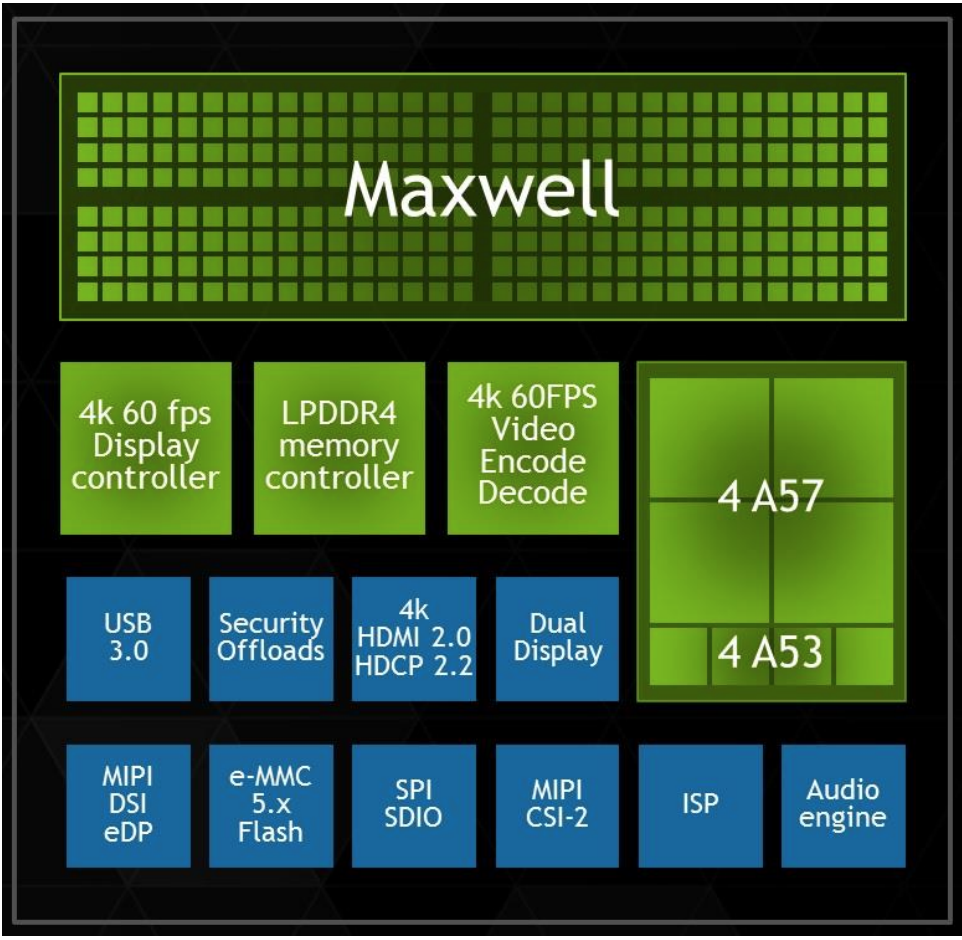
\includegraphics[width=0.5\textwidth]{tx1}
	\caption{Jetson TX1 硬件架构图}
	\label{fig:tx1}
\end{figure}

\subsection{Darknet}
VGG16网络包含13个卷积层,3个全连接层以及5个池化层(不含参数),共计约132M个参数,占用存储空间528MB,对于$224\times224$大小的输入图像执行约30.94 Billion次运算。若Atrous Faster R-CNN选用VGG16作为基础网络显然不能在Jetson TX1上实时运行,而且功耗很高,因为需要很多次的内存读操作,而内存读写操作比ALU计算单元的功耗要大得多,约为100:1。因此,我们必须使用比较小的模型来减少模型参数和计算量,并保证目标检测精度不会出现显著降低。本文采用了DarkNet这种网络结构,它可以看作精简版的VGG16网络,与VGG16、AlexNet的对比见表 \ref{tab:nets}。
\begin{table}
	\caption{AlexNet、VGG16、Darknet在ImageNet 2012图像分类上的表现以及网络规模对比,表中``Bn''表示``BIllion'',``MB''表示``Mega Bytes''。}
	\centering
	\begin{tabular}{ccccc}
		\toprule
		模型 & Top-1 & Top-5 & 计算次数 & 存储\\
		\midrule
		AlexNet & 57.0 & 80.3 & 2.27 Bn & 285 MB\\
		VGG16 & 70.5 & 90.0 & 30.94 Bn & 528 MB\\
		Darknet & 61.1 & 83.0 & 0.81 Bn & 28 MB\\
		\bottomrule		
	\end{tabular}	
	\label{tab:nets}
\end{table}

从表 \ref{tab:nets}可以看出Darknet在精度与网络规模之间作出了很好的权衡,Darknet的网络结构如图 \ref{fig:darknet}所示,下文将Darknet的卷积层依次称为\texttt{conv1},\texttt{conv2},$\cdots$,\texttt{conv8},特征图的维度分别为16,32,64,128,256,512,1024,1000,MAX池化层依次称为\texttt{pool1},\texttt{pool2},$\cdots$,\texttt{pool6}。Darknet是一个全卷积神经网络,而且使用了Batch Normalization \cite{batch-norm}来加速训练过程。为了使用Darknet作为Atrous Faster R-CNN的基础网络,我们需要将Darknet分为两部分:卷积网络与RoI网络。为此我们对Darknet进行如何变换:
\begin{namelist}{}
	\item
	(1)将\texttt{pool5} MAX池化层换成网格大小为$7\times7$的RoI池化层;
	\item
	(2)用两个同级的卷积层替换\texttt{conv8},这两个卷积层分别用来做分类和边框回归,卷积核大小分别为$3\times3\times21$,$3\times3\times84$,并且在这两个卷积层后分别加一个Average池化层。
	\item
	(3)在\texttt{conv5}后接第\ref{chap:2}章中提出的Atrous Region Proposal Network,并将位置编码的维度由512变成256以减少计算量。
\end{namelist}
除了对网络结构进行上述变换,其他因素例如损失函数选取、样本采样方式等均保持不变。精简版的Atrous Faster R-CNN在Jetson TX1上运行速率为15 \texttt{fps},在PASCAL VOC 2007测试集上的检测精度为57.1\%(mAP)。
\begin{figure}[h]
	\centering
	\includegraphics[width=\textwidth]{darknet}
	\caption{Darknet网络,图中红色表示MAX池化层,黑色表示卷积层,所有卷积核的空间大小都是$3\times3$,图中省略了每个卷积层后的BatchNorm层。}
	\label{fig:darknet}
\end{figure}

\section{提升检测精度}
在上一节中我们将Atrous Faster R-CNN网络进行裁剪并移植到了Jetson TX1嵌入式平台,并且能够获得15 \texttt{fps}的运行速率,但是检测器的准确度明显下降了(从76.9\%下降到57.1\%)。这一小节中运用两个小技巧在不增加任何计算量的前提下提升精简版Atrous Faster R-CNN的检测精度。

\subsection{多层特征融合}
第\ref{chap:2}章中提出的Atrous Region Proposal Network(ARPN)通过具有不同感知野的分支去预测不同尺度的候选区域,并且实验证明该方法的性能优于Region Proposal Network。ARPN中不同的分支共享\texttt{conv5\_3}卷积特征图,但\texttt{conv5\_3}卷积特征图属于高层的特征空间,很难保留物体的细节特征。这对小物体的检测以及遮挡物体的定位都会带来不利的影响。图像语义分割中常常使用特征融合的方法,即把浅层的特征与高层的特征经过尺度变换后拼在一起。拼接的方式基本有两种,一种是像GoogLeNet \cite{inception-v4}一样,按channel维度拼起来,第二种像ResNet \cite{resnet}那样,把它们直接相加。现在这种做法也变成了趋势,越来越多人做视觉任务都用了类似的方法。经过多层卷积,下采样后得到低分辩的高维表达,可以抽象出物体的高层语意表达,捕获物体的上下文空间信息,相当于是一个bottom-up的表达抽象过程。然后再逐步把前面的特征组合起来,补充细节信息,这相当于再做一个top-down的修正。

将低分辩率的高层特征经过尺度放大与高分辨率的浅层特征融合会增大滑动特征图的分辨率,进而增大运算量,而且需要归一化各层特征的激活值,通常需要精心设置学习率。因此本文采用了一种``late fusion''的方案来提取多尺度的候选区域:直接在不同层的特征上预测不同大小的候选区域,然后将所有这些候选窗口放在一起做非极大值移植(NMS),然后选取前$N$个候选窗口。具体来说,我们仍然使用VGG16作为基础网络,使用 \texttt{conv4\_3}的特征预测尺度为64,128的anchors的边框回归以及前景概率,使用 \texttt{conv5\_3}的特征预测尺度为256,512的anchors。正如ParseNet \cite{parsenet}中所指出的那样,\texttt{conv4\_3}的特征值要比比\texttt{conv5\_3}的特征值大很多,这通常会导致网络难以训练,因此本文采用L2 Normalization的方法对\texttt{conv4\_3}的特征值进行归一化处理。对于一个给定的$d$维特征向量$\rm{x}=(x_1\dots x_d)$,L2 Normalization对它进行如下操作:
\begin{equation}
\begin{aligned}
\hat{\rm{x}} &= \frac{\rm{x}}{||\rm{x}||_2} \\
y_i &= \gamma_i \hat{x}_i
\end{aligned}
\end{equation}
其中$||\rm{x}||_2$表示特征向量$\rm{x}$的L2范数,$\gamma_1,\dots, \gamma_d$表示可学习的缩放系数,初始值均设置为20,也就是说\texttt{conv4\_3}特征经过归一化后的L2范数初始化为20,网络结构如图\ref{fig:arpn-v2}所示。
\begin{figure}[h]
	\centering
	\includegraphics[width=\textwidth]{arpn-v2}
	\caption{ARPN V2网络结构示意图}
	\label{fig:arpn-v2}
\end{figure}

在ARPN的训练过程中,与ground-truth边界框交并比(IoU)超过0.7或者对某一ground truth边界框而言与它拥有最大交并比的anchor被选为前景区域(图\ref{fig:fg-bg}中红色区域),与所有ground truth的交并比都小于0.3的anchor被选为背景区域(图\ref{fig:fg-bg}中黑色区域),其他的anchor(图\ref{fig:fg-bg}中灰色区域)不参与训练。训练时对前景区域和背景区域同时做分类,但只对前景区域做边界框回归。但是,ARPN测试阶段可能会将位于灰色区域的anchor分类为前景,由于训练过程中没有学习到如何对这类区域进行边界框回归,此时得到的候选框的位置便有可能是不准确的。因此我们对灰色区域的样本也进行边界框回归,这么做的目的是希望ARPN即使把灰色区域当成正样本,那么此时得到的边界框位置也是准确的。实验证明这个小技巧能够提高生成的候选区域的质量。
\begin{figure}[h]
	\centering
	\includegraphics[scale=1]{fg-bg}
	\caption{前景背景示意图,红色表示前景区域,黑色表示背景区域。}
	\label{fig:fg-bg}
\end{figure}
经过多层特征融合以及中间区域边界框回归,精简版Atrous Faster R-CNN的检测精度有所提升(从57.1\%提升到59.3\%)。
\section{难分样本挖掘}
Atrous Faster R-CNN对每幅图像提取大约2000个候选区域(RoIs)用于训练。这大约2000个候选区域中前景和背景(不包含任意感兴趣的目标)的分布高度不均衡,绝大部分的候选窗口都是背景,极端情况下背景候选区域和前景候选区域的比例能够达到$100:1$。Atrous Faster R-CNN采用与Fast R-CNN相同的策略来处理这种样本不均衡问题,即在每个minibatch中对背景候选区域随机采样使得正负候选区域的比例能够达到$1:3$。这种简单的处理策略在一定程度上缓解了样本不均衡问题,但是也引入了一些需要手工调节与试凑的参数,与此同时在线难分样本挖掘(online hard example mining)的方法最近被证实对样本不均衡问题很有效 \cite{ohem} \cite{densebox}。

挖掘难分样本的技术即bootstrapping,先构造一个初始训练集,完成迭代训练后固定模型寻找错分样本,然后利用这些错分样本重新构造训练集迭代训练更新模型并寻找错分样本,如此循环往复。其实以前大家在用boosting,DPM等方法的时候已经这么做了,Felzenszwalb证实在DPM中通过bootstrapping SVM可以在整个数据集上找到最优的分类策略。Fast R-CNN以及它的变体之所以没有使用bootstrapping策略,主要的困难在于:boostrapping的两个阶段是,使用固定模型寻找错分样本,使用错分样本训练新的模型。训练深度卷积检测器时需要数以万计次的SGD迭代,如果在某个阶段固定模型参数会拖慢训练过程。

为了不拖慢深度CNN网络的训练过程,Shrivastava等 \cite{ohem}提出了在线难分样本挖掘(online hard example mining, OHEM)技术。OHEM对SGD过程进行了一些调整,训练样本不使用固定的分布采样,而是根据每个样本当前的损失值来决定要不要把它加入训练集。在Fast R-CNN中使用OHEM的详细过程如下:在第$t$次SGD迭代过程中,首先进行卷积网络的计算得到卷积特征图,之后RoI网络使用这个卷积特征图以及所有的RoIs进行前向传播,获得每个RoI的损失值,并根据损失值对所有的RoIs进行排序,选择前$B$个损失值最高的RoIs进行反向传播计算梯度。

实验过程中,我们使用所有经过非极大值抑制(阈值设置为0.7)后的proposal进行前向计算,然后选择损失值最高的前128个进行反向传播计算梯度。采用难分样本挖掘将目标检测算法的检测精度提升了1.7\%。本章将第 \ref{chap:2} 中提出的目标检测算法移植到嵌入式的Jetson TX1开发平台上,为此对网络结构进行了精简以适应嵌入式设备的存储和计算资源,并采用了两个工程上的trick进一步提升了在嵌入式平台上目标检测的精度。